%\begin{frame}
%\frametitle{Model: Overview}
%\begin{center}
%\begin{tikzpicture}[->]
%	% draw input layer
%	\foreach \s in {0,...,7}
%	{
%		\node[draw, circle] (i_\s) at (0,-\s * 0.5) {};
%	}
%	
%	% draw output layer	
%	\foreach \s in {0,...,2}
%	{
%		\node[draw, circle] (o_\s) at (3,-1.25 -\s * 0.5) {};
%		\node (m_\s) at (5,-1.25 -\s * 0.5) {};
%		\path (o_\s) edge node {} (m_\s);
%	}
%	
%	% draw edges
%	\foreach \s in {0,...,7}
%	{
%			\path (i_\s) edge node {} (o_0);
%	}
%	\path (i_0) edge node {} (o_1);
%	\path (i_0) edge node {} (o_2);
%
%	% draw underbraces and labels
%	\node[] (l_0) at (0,-4) {$\underbrace{\ }$};
%	\node[] (l_0) at (0,-4.5) {\scriptsize{input layer}};
%	\node[] (l_0) at (1.5,-4) {$\underbrace{\ \ \ \ \ \ \ \ \ \ \ \ \ \ \ \ \ }$};
%	\node[] (l_0) at (1.5,-4.5) {\scriptsize{weights}};
%	\node[] (l_0) at (3,-4) {$\underbrace{\ }$};
%	\node[] (l_0) at (3,-4.5) {\scriptsize{output layer}};
%\end{tikzpicture}
%\end{center}
%\end{frame}

\begin{frame}
\frametitle{Model: Overview}
\begin{center}
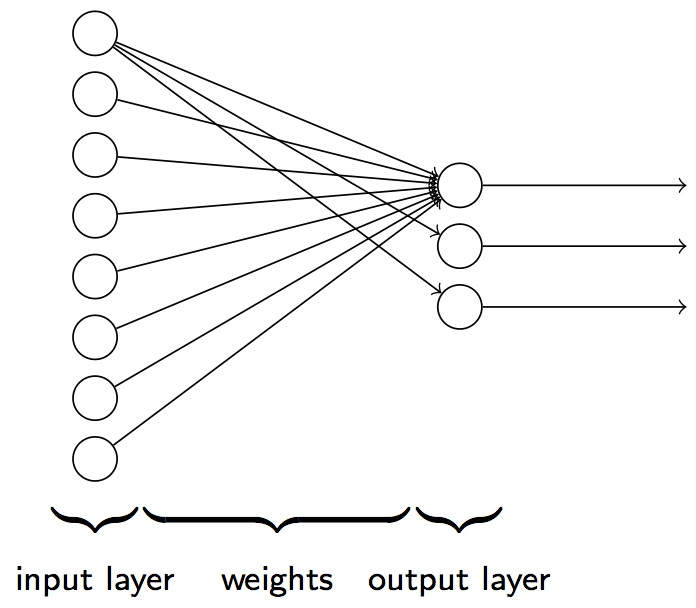
\includegraphics[scale=0.3]{pics/model_overview}
\end{center}
\end{frame}

\begin{frame}
\frametitle{Model: Input Layer}
\begin{tikzpicture}[overlay,remember picture]
\node[anchor=north west] at ($(current page.north west)+(0,-1)$) {
  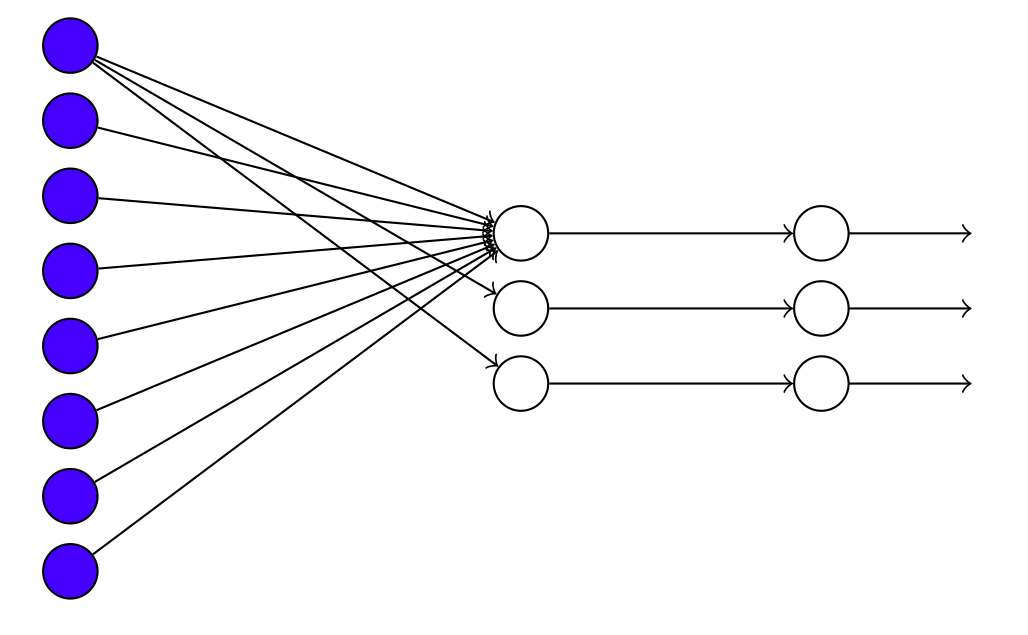
\includegraphics[scale=.1]{pics/model_input}
};
\node[anchor=north east] at ($(current page.north east)+(-2,-1.5)$) {
  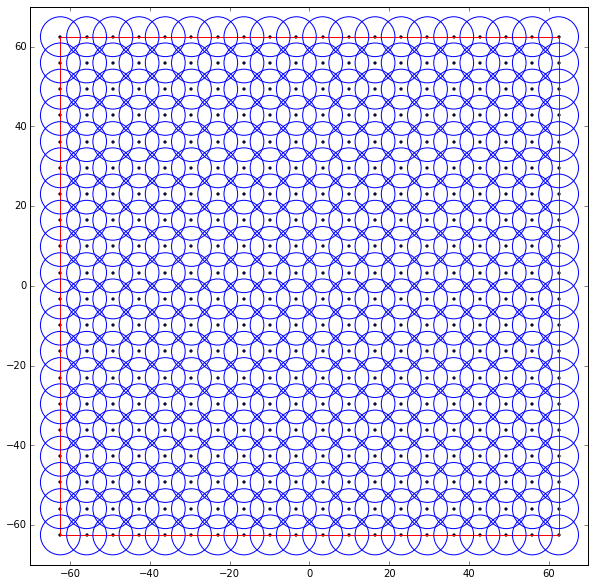
\includegraphics[scale=.2]{pics/place_cell_locations}
};
\node[anchor=south west] at ($(current page.south west)+(1,1)$) {
  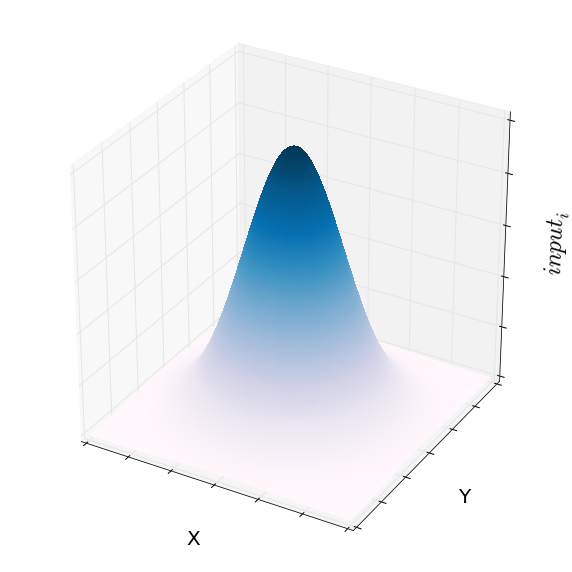
\includegraphics[scale=.2]{pics/gauss}
};
\node[anchor=south east] at ($(current page.south east)+(-1.5,2)$) {
  \footnotesize{$input_i = \exp(-\frac{||rat\_pos - center_i||^2}{50})$}
};
\end{tikzpicture}
\end{frame}


\begin{frame}
\frametitle{Model: Input Layer}
\begin{tikzpicture}[overlay,remember picture]
\node[anchor=north west] at ($(current page.north west)+(0,-1)$) {
  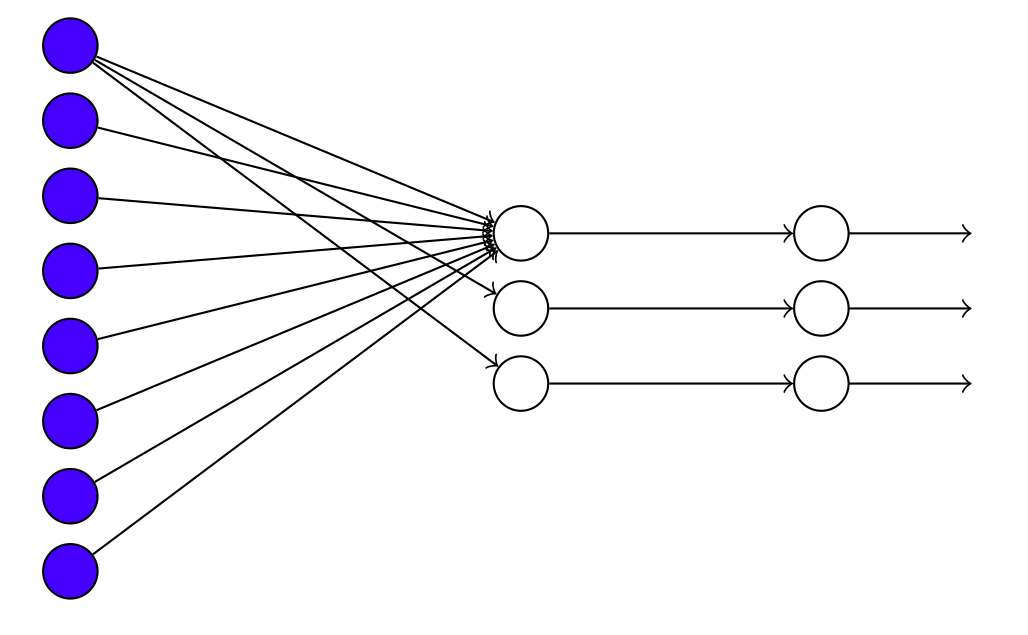
\includegraphics[scale=.1]{pics/model_input}
};
\node[anchor=north east] at ($(current page.north east)+(-1.5,-1.5)$) {
  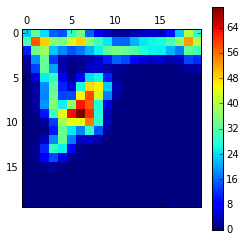
\includegraphics[scale=.55]{pics/activity_demo}
};
\node[anchor=south west] at ($(current page.south west)+(1,1)$) {
  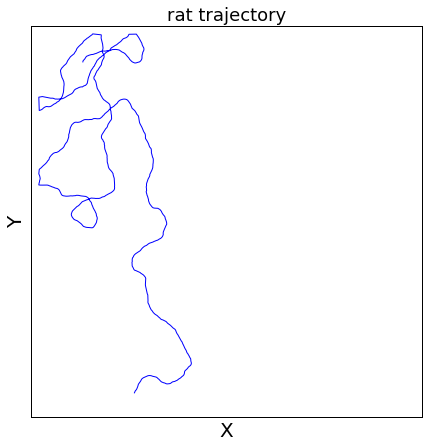
\includegraphics[scale=.27]{pics/mouse_demo}
};
\end{tikzpicture}
\end{frame}

\begin{frame}
\frametitle{Model: Output Layer}
\begin{tikzpicture}[overlay,remember picture]
\node[anchor=north west] at ($(current page.north west)+(0,-1)$) {
  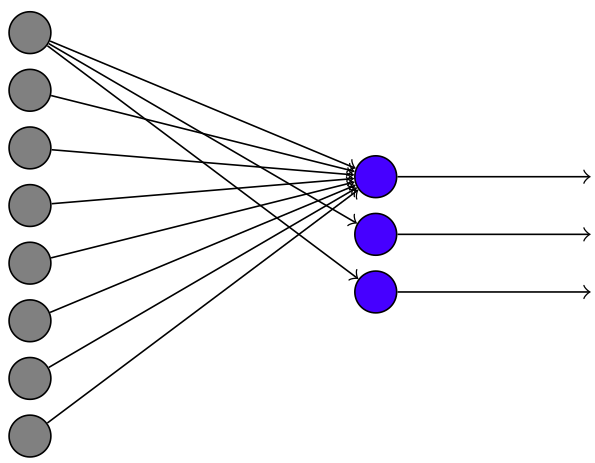
\includegraphics[scale=.1]{pics/model_output}
};
\node[anchor=north east] at ($(current page.north east)+(-2,-1.5)$) {
  $h_j(t) = \sum_i w_{ij} \cdot input_i(t)$
};
\end{tikzpicture}
\end{frame}

\begin{frame}
\frametitle{Model: Output Layer}
\begin{tikzpicture}[overlay,remember picture]
\node[anchor=north west] at ($(current page.north west)+(0,-1)$) {
  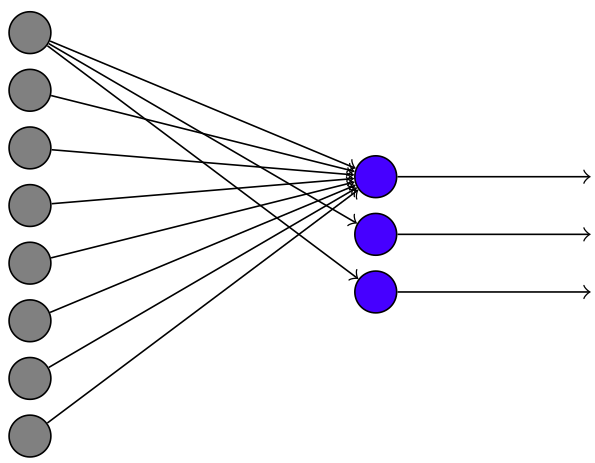
\includegraphics[scale=.1]{pics/model_output}
};
\node[anchor=north east] at ($(current page.north east)+(-2,-1.5)$) {
  $h_j(t) = \sum_i w_{ij} \cdot input_i(t)$
};
\node[anchor=north east] at ($(current page.north east)+(-3,-4)$) {
  $\rightarrow$ adaptation dynamics:
};
\node[anchor=north east] at ($(current page.north east)+(-1.1,-4.7)$) {
  $\tau^+\frac{d}{dt}r^+_j(t)=h_j(t)-r^+_j(t)-r^-_j(t)$
};
\node[anchor=north east] at ($(current page.north east)+(-3.7,-5.6)$) {
  $\tau^-\frac{d}{dt}r^-_j(t)=r^-_j(t)$
};
\node[anchor=north west] at ($(current page.north west)+(0.5,-3.5)$) {
  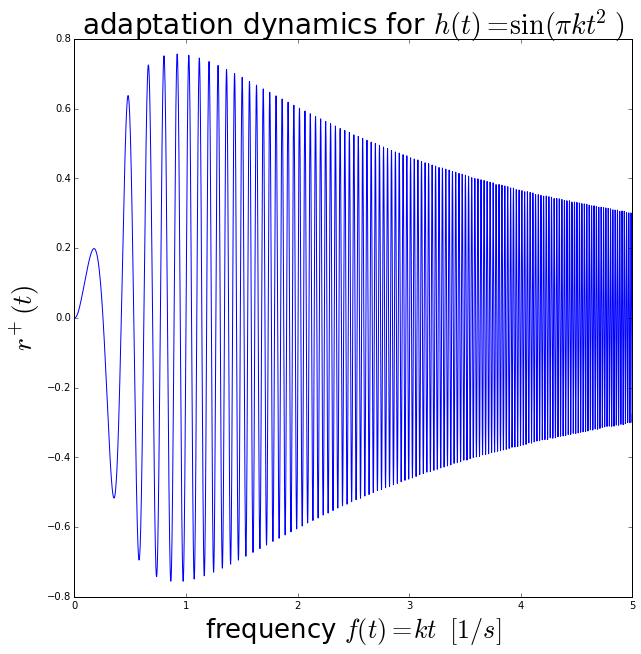
\includegraphics[scale=.2]{pics/sinusoidal_activation}
};
\end{tikzpicture}
\end{frame}

\begin{frame}
\frametitle{Model: Output Layer}
\begin{tikzpicture}[overlay,remember picture]
\node[anchor=north west] at ($(current page.north west)+(0,-1)$) {
  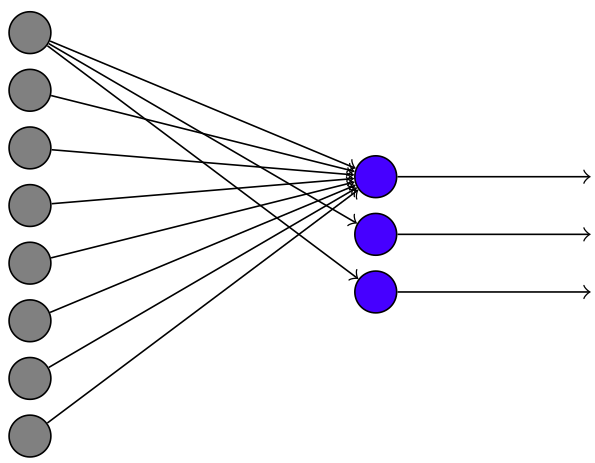
\includegraphics[scale=.1]{pics/model_output}
};
\node[anchor=north east] at ($(current page.north east)+(-3,-1.7)$) {
  $\rightarrow$ solution $r^+_j(t)$
};
\node[anchor=north east] at ($(current page.north east)+(-1.5,-4.5)$) {
  $output_j(t) = F(r^+_j(t);g(t),\mu(t))$
};
\node[anchor=north east] at ($(current page.north east)+(-3.2,-5.6)$) {
  $g(t)$ - gain
};
\node[anchor=north east] at ($(current page.north east)+(-2.7,-6.5)$) {
  $\mu(t)$ - threshold
};
\node[anchor=north west] at ($(current page.north west)+(0.5,-3.5)$) {
  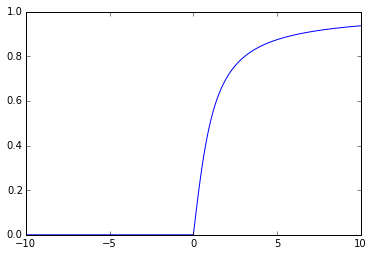
\includegraphics[scale=.2]{pics/output_function}
};
\end{tikzpicture}
\end{frame}


\begin{frame}
\frametitle{Model: Weight Updates}
\begin{tikzpicture}[overlay,remember picture]
\node[anchor=north west] at ($(current page.north west)+(0,-1)$) {
  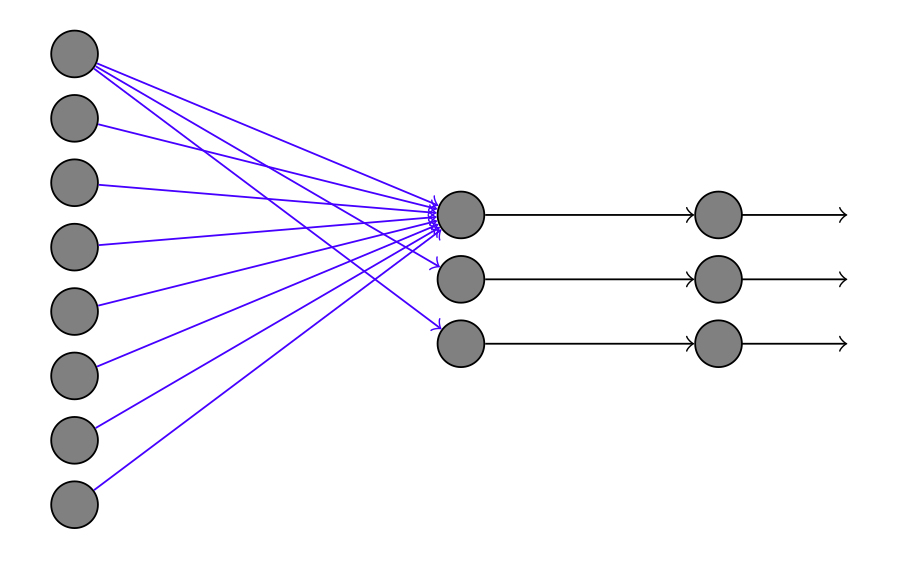
\includegraphics[scale=.1]{pics/model_weights}
};
\node[anchor=north east] at ($(current page.north east)+(-2.1,-1.7)$) {
  $h_j(t) = \sum_i w_{ij} \cdot input_i(t)$
};
\node[anchor=north west] at ($(current page.north west)+(1,-4)$) {
  How to determine the weights $w_{ij}$?
};
\end{tikzpicture}
\end{frame}


\begin{frame}
\frametitle{Model: Weight Updates}
\begin{tikzpicture}[overlay,remember picture]
\node[anchor=north west] at ($(current page.north west)+(0,-1)$) {
  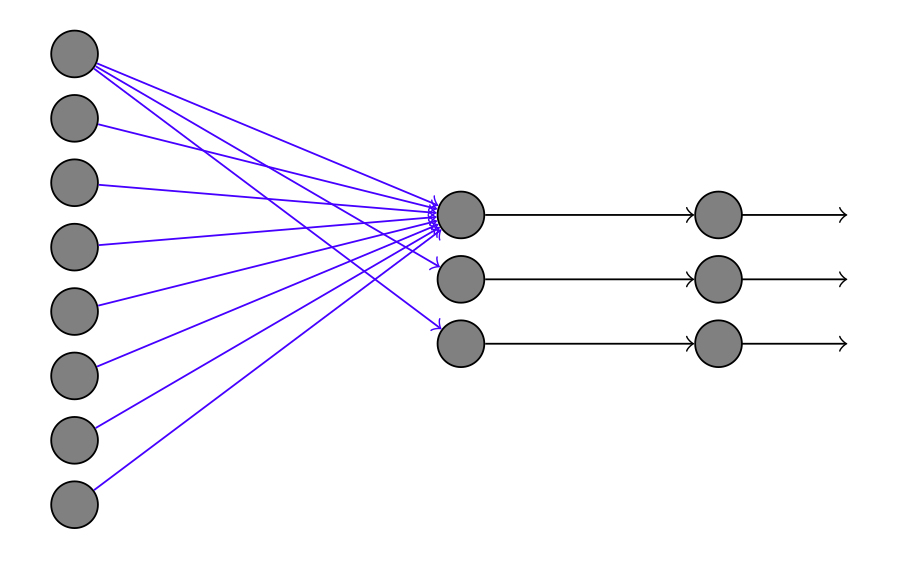
\includegraphics[scale=.1]{pics/model_weights}
};
\node[anchor=north east] at ($(current page.north east)+(-2.1,-1.7)$) {
  $h_j(t) = \sum_i w_{ij} \cdot input_i(t)$
};
\node[anchor=north west] at ($(current page.north west)+(1,-4)$) {
  How to determine the weights $w_{ij}$?
};
\node[anchor=north west] at ($(current page.north west)+(1,-4.7)$) {
  $\rightarrow$ Hebbian learning dynamics ('Fire together, wire together')
};
\node[anchor=north west] at ($(current page.north west)+(1,-6)$) {
  $w_{ij}(t+\Delta t) = w_{ij}(t) + \epsilon(input_i(t)\cdot output_j(t) - \overline{input_j} \cdot \overline{output_j})$
};
\end{tikzpicture}
\end{frame}
